% \documentclass{book}

\documentclass[12pt]{article}
\usepackage[pdfborder={0 0 0.5 [3 2]}]{hyperref}%
\usepackage[left=1in,right=1in,top=1in,bottom=1in]{geometry}%
\usepackage[shortalphabetic]{amsrefs}%
\usepackage{amsmath}
\usepackage{enumerate}
\usepackage{enumitem}
\usepackage{amssymb}                
\usepackage{amsmath}                
\usepackage{amsfonts}
\usepackage{amsthm}
\usepackage{bbm}
\usepackage[table,xcdraw]{xcolor}
\usepackage{tikz}
\usepackage{float}
\usepackage{booktabs}
\usepackage{svg}
\usepackage{mathtools}
\usepackage{cool}
\usepackage{url}
\usepackage{graphicx,epsfig}
\usepackage{makecell}
\usepackage{array}

\def\noi{\noindent}
\def\T{{\mathbb T}}
\def\R{{\mathbb R}}
\def\N{{\mathbb N}}
\def\C{{\mathbb C}}
\def\Z{{\mathbb Z}}
\def\P{{\mathbb P}}
\def\E{{\mathbb E}}
\def\Q{\mathbb{Q}}
\def\ind{{\mathbb I}}

\graphicspath{ {images8/} }

\begin{document}

\section*{2 March 2017}
From a series of trials I did, I concluded that (for now), Fourier spectral methods do not converge in a useful manner. I tried Fourier methods on a system for which I knew the spectrum (1D Laplace equation with periodic BCs), and increasing number of nodes actually makes things worse after a point. The documentation for the \textrm{fourdif} Matlab code suggests you shoudn't be using this for too many nodes. So I decided to not use Fourier for now.\\

To avoid the extra Neumann eigenvalue, I decided to use finite difference methods with periodic boundary conditions. I used the following paramaters:
\begin{enumerate}
	\item Domain length $L = 100$. For shorter domains, there are some weird boundary effects even with the known solution, so avoid this I chose a value I deemed sufficiently large to make this irrelevant.
	\item Continuation code was run to $c = 40.9355$. This was arbitrary, but I wanted to make sure we eigenvalues were sufficiently large. To the extent that I have looked, eigenvalues increase in magnitude with increasing $c$.
	\item Grid points range from $N = 2500 - 40000$. For less that 2500, we get weird eigenvalue results, and fsolve does not find a solution for more than 40000.
\end{enumerate}

\subsection*{Double pulse 1}
We start with constructing the first double pulse as before. We already know that we should have a pair of real eigenvalues which are negatives of each other, but it is nice to verify. Here is a plot of the the pulse together with its eigenvalues.
\begin{figure}[H]
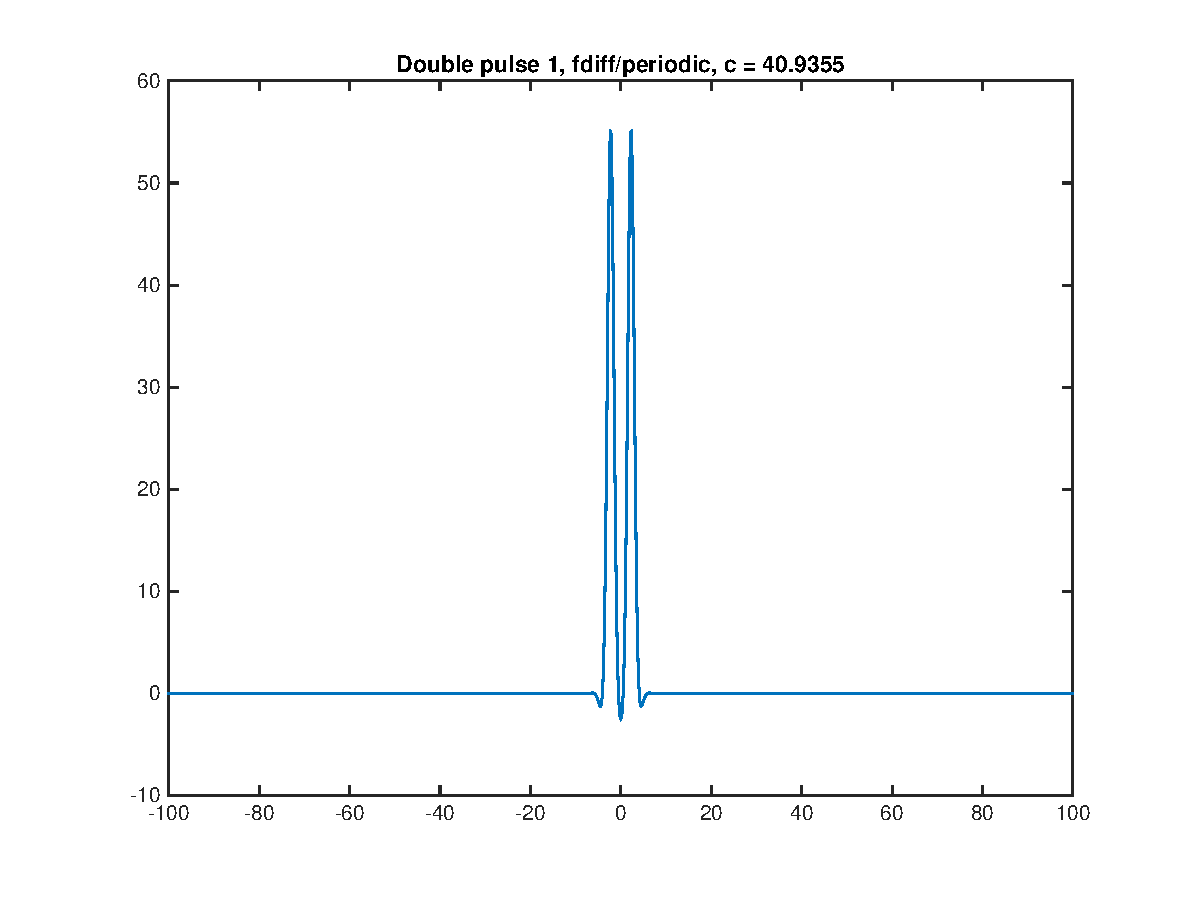
\includegraphics[width=8.5cm]{double1.eps}
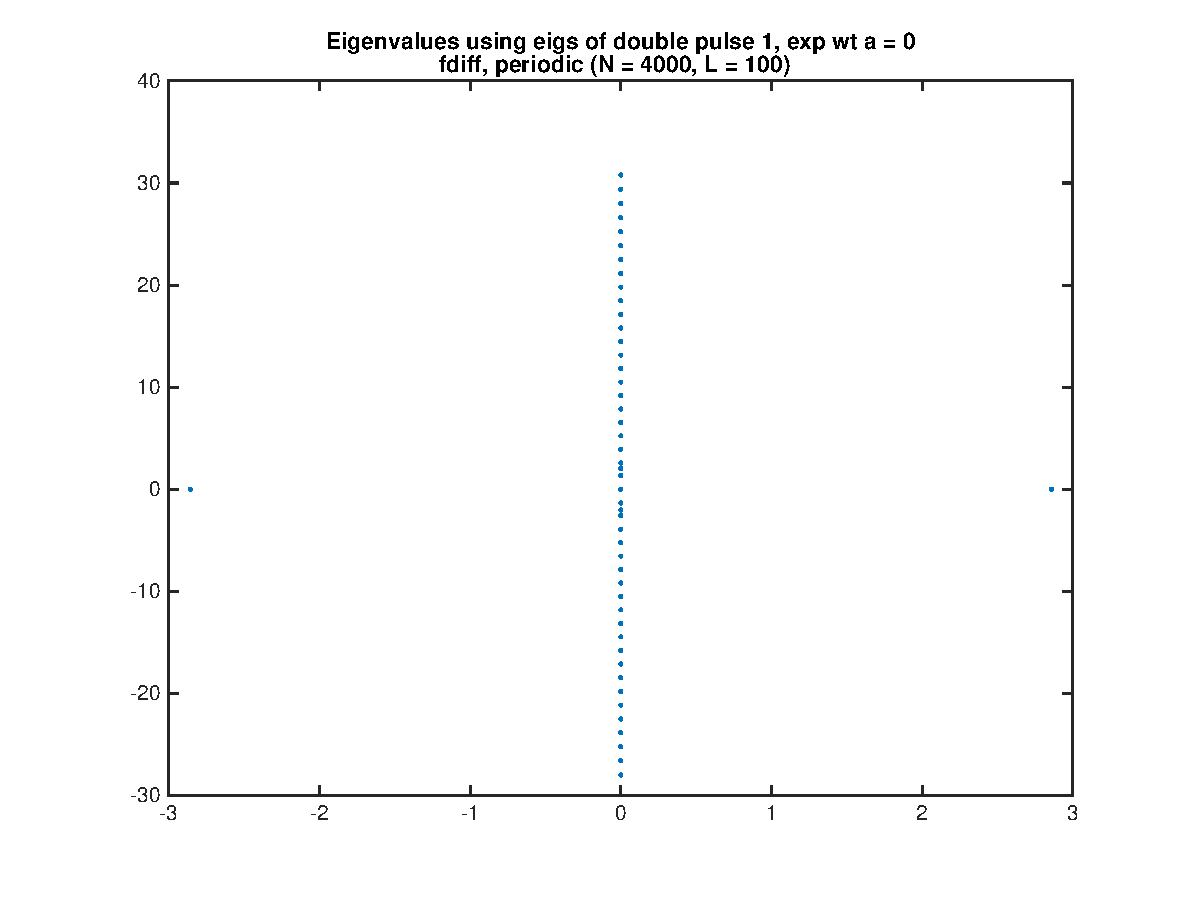
\includegraphics[width=8.5cm]{double1eigs.eps}
\end{figure}
Now we look at the rightmost (real) eigenvalue for different values of N:

\begin{figure}[H]
\begin{tabular}{l|ll}
$N$       & Rightmost eigenvalue & Change (from prev) \\ \hline
4000      &   2.8573 &            \\
8000      &   3.3513 &   0.4940   \\
16000     &   3.4627 &   0.1115   \\
32000     &   3.4900 &   0.0272   \\
64000     &   3.4966 &   0.0066   \\       
\end{tabular}
\end{figure}
Plotting the log of the change versus the log of the stepsize $h = 200/N$ (taking the coarser stepsize for the plot), we get a nice straight line with order of convergence approximately 2.
\begin{figure}[H]
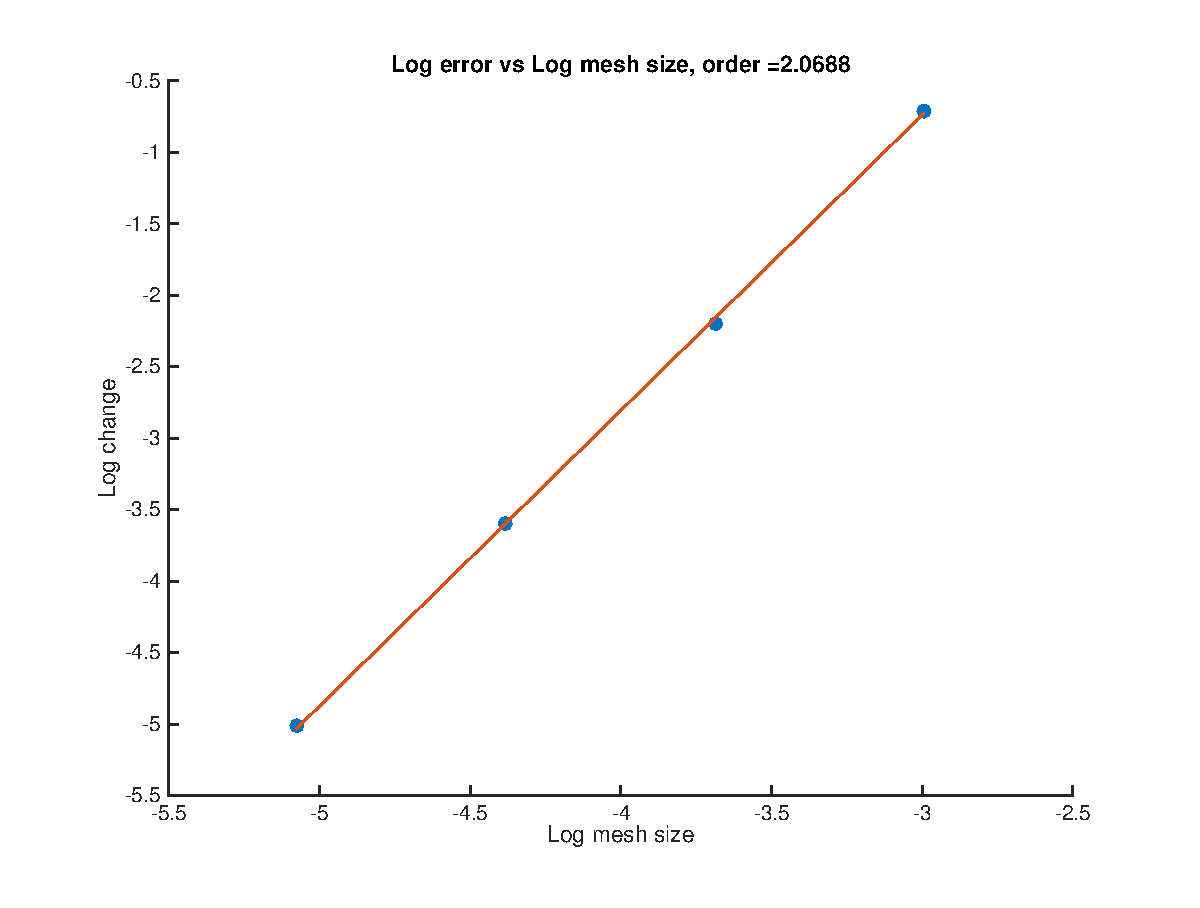
\includegraphics[width=8.5cm]{double1logplot1.eps}
\end{figure}
Using a geometric series and a little guesswork, we reason that this is converging to a true value of appromately $3.4986$. Testing this out with an error plot, we get another nice straight line with the same order of convergence.
\begin{figure}[H]
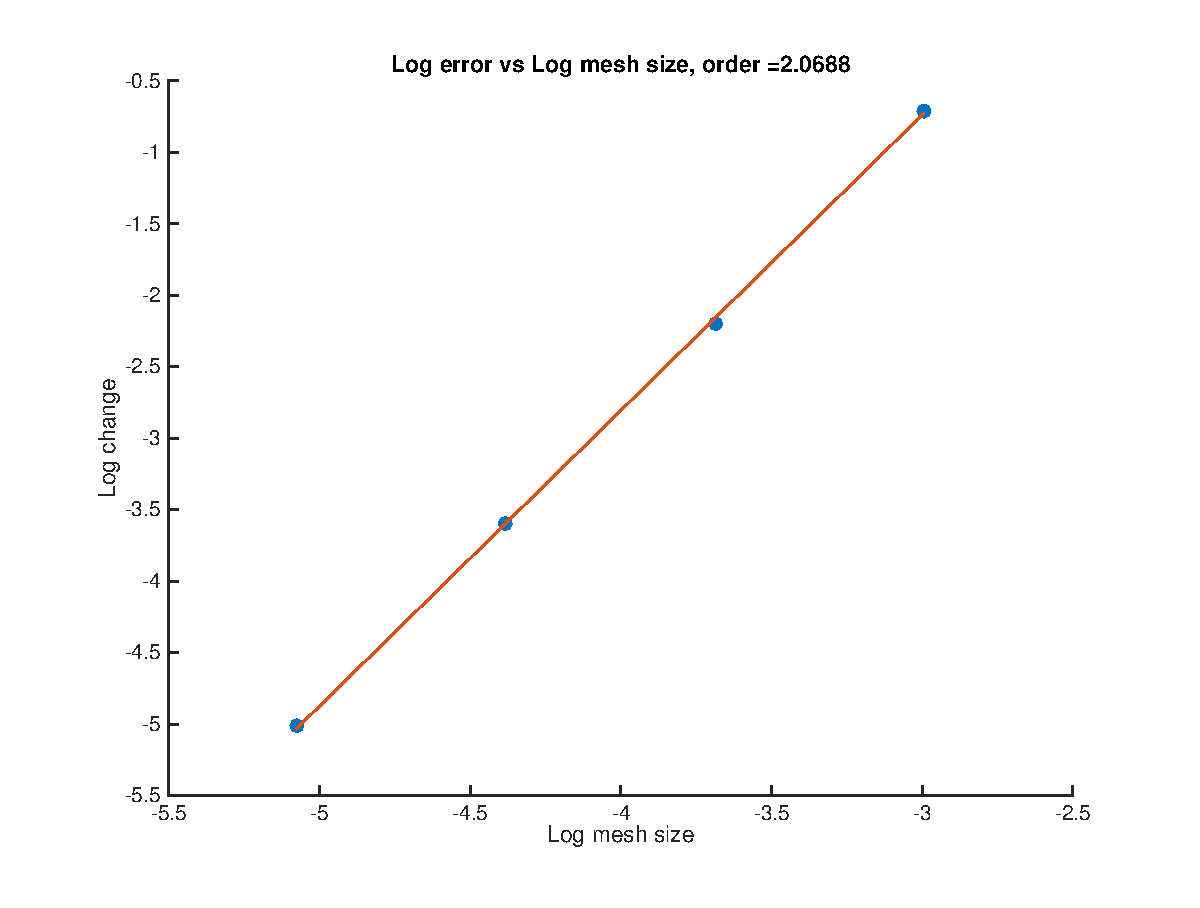
\includegraphics[width=8.5cm]{double1logplot1.eps}
\end{figure}

\subsection*{Double pulse 2}
This is the one we really care about. Here is a plot of it along with its a zoom of its eigenvalues in an exponentially weighted space with weight $a = 0.25$. This weight was chosen to give good separation from the essential spectrum and good convergence of eigenvalues. The essential spectrum (not shown) is moved left to about $x = -10$, so separation is good. Picture is $N = 4000$.
\begin{figure}[H]
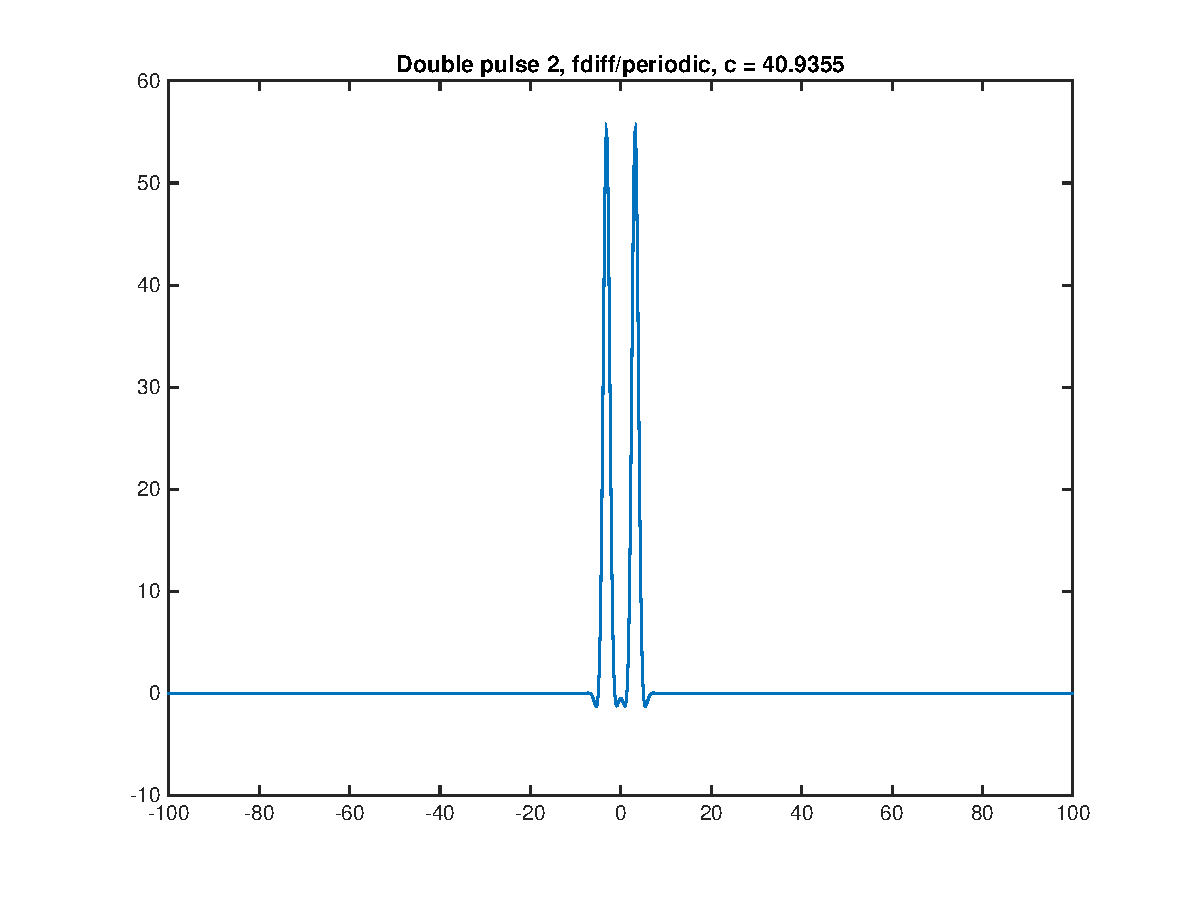
\includegraphics[width=8.5cm]{double2.eps}
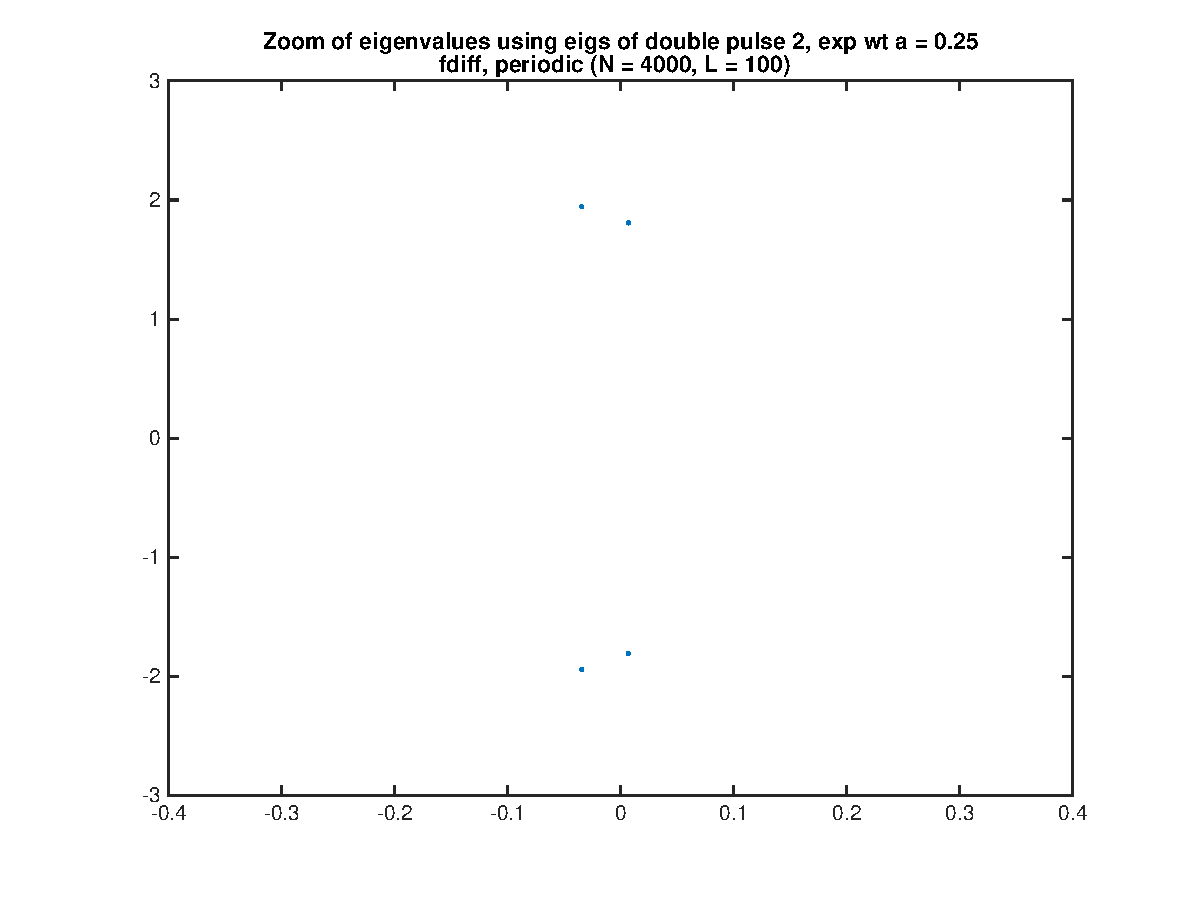
\includegraphics[width=8.5cm]{double2eigszoom.eps}
\end{figure}
From the eigenvalue picture, we can tell nothing about what the eigenvalues will be, since they will move as we change the number of grid points. We will do the same thing we did above. We take the eigenvalues with positive imaginary part and track them as we increase the number of grid points. When we do this, we check the eigenfunctions to make sure we are tracking the correct eigenvalue. Since we don't know what is going on yet, we will refer to these eigenvalues as the left eigenvalue and the right eigenvalue, indicating their position on the plot above. Here is a table of these eigenvalues for increasing $N$.

Table of eigenvalues:
\begin{figure}[H]
\begin{tabular}{l|ll}
$N$     & Left eigenvalue     &  Right eigenvalue  \\ \hline
2500    &  -0.0663 - 3.0131i  & -0.0078 - 2.8746i  \\
5000    &  -0.0239 - 1.5987i  &  0.0063 - 1.4498i  \\
10000   &  -0.0064 - 0.9722i  &  0.0021 - 0.7276i  \\
20000   &  -0.0016 - 0.7386i  &  0.0005 - 0.3641i  \\
40000   &  -0.0005 - 0.6679i  &  0.0000 - 0.1827i  \\       
\end{tabular}
\end{figure}

First we hypothesize that the right eigenvalue is the zero eigenvalue since its eigenfunction looks like an exponentially scaled version of the derivative of the double pulse. To verify this, we plot the log of its absolute value versus the log of the mesh size $h = 200/N$.
\begin{figure}[H]
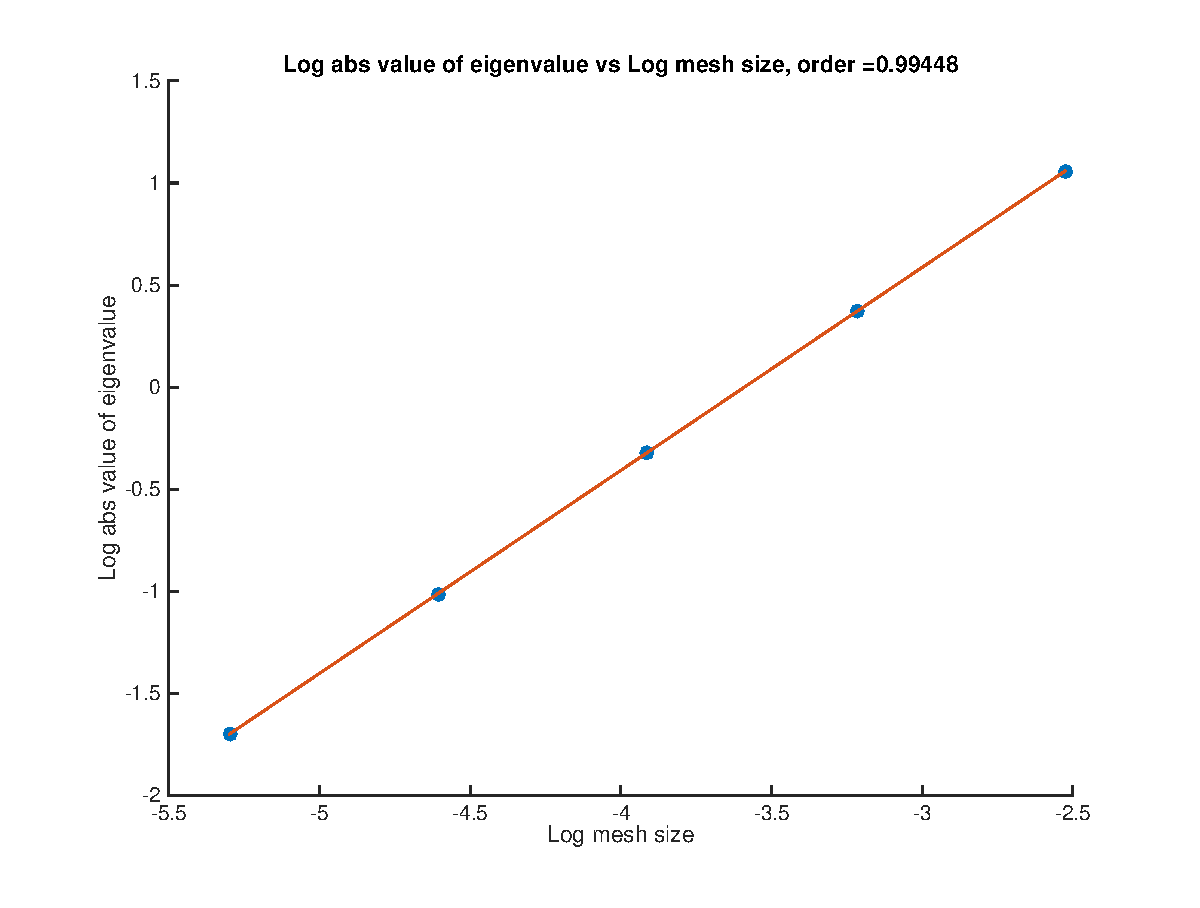
\includegraphics[width=8.5cm]{double2logplotright.eps}
\end{figure}
We get a nice straight line (although only 1st order convergence), so we conclude that these are the zero eigenvalues. \\

For the left eigenvalue, we hypothesize that it will converge to the imaginary axis, so first we plot the log of the real part versus the log of the mesh size.
\begin{figure}[H]
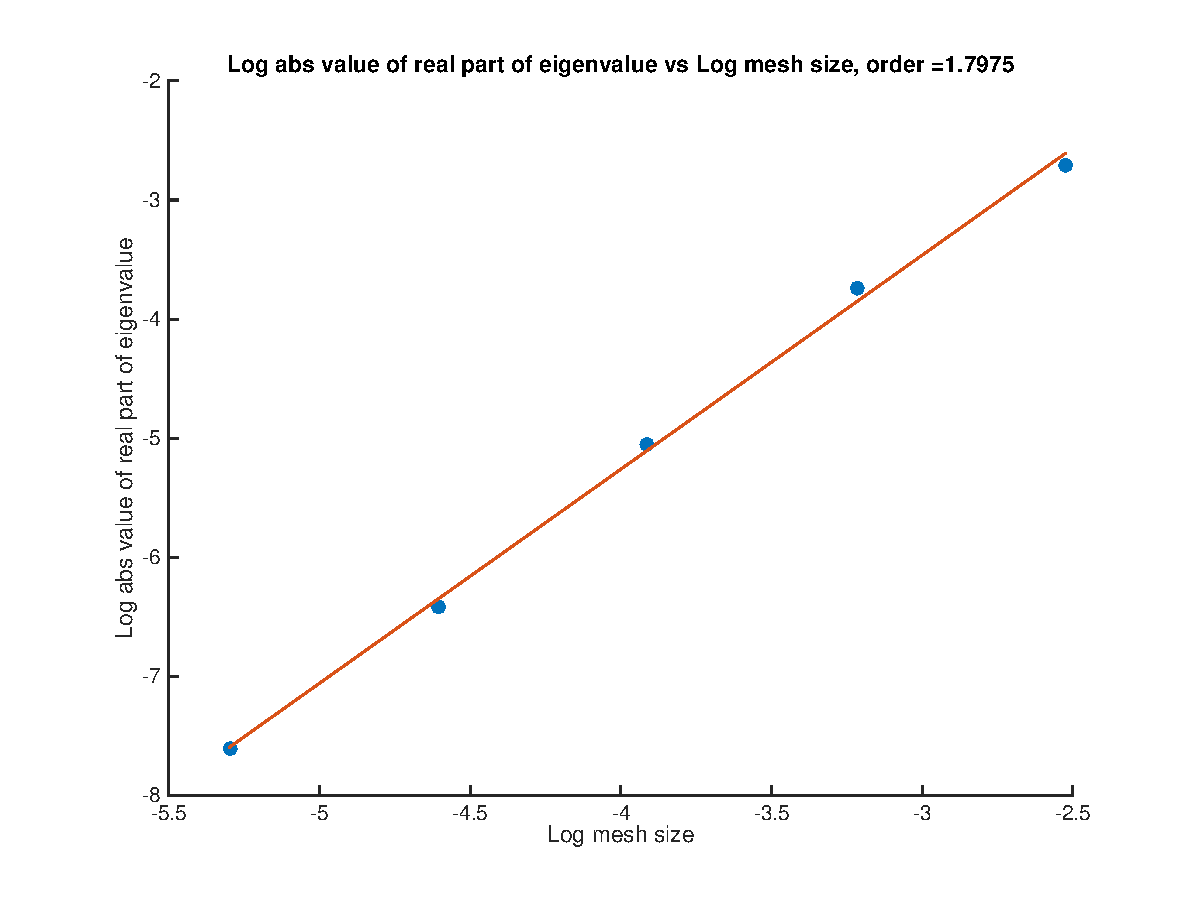
\includegraphics[width=8.5cm]{double2logplotleftreal.eps}
\end{figure}
It's not as nice as the straight line above, but it's pretty good. At least it is reasonable to me that the real part converges to 0. For the imaginary part, we do the same thing we did above and plot the change versus grid size.
\begin{figure}[H]
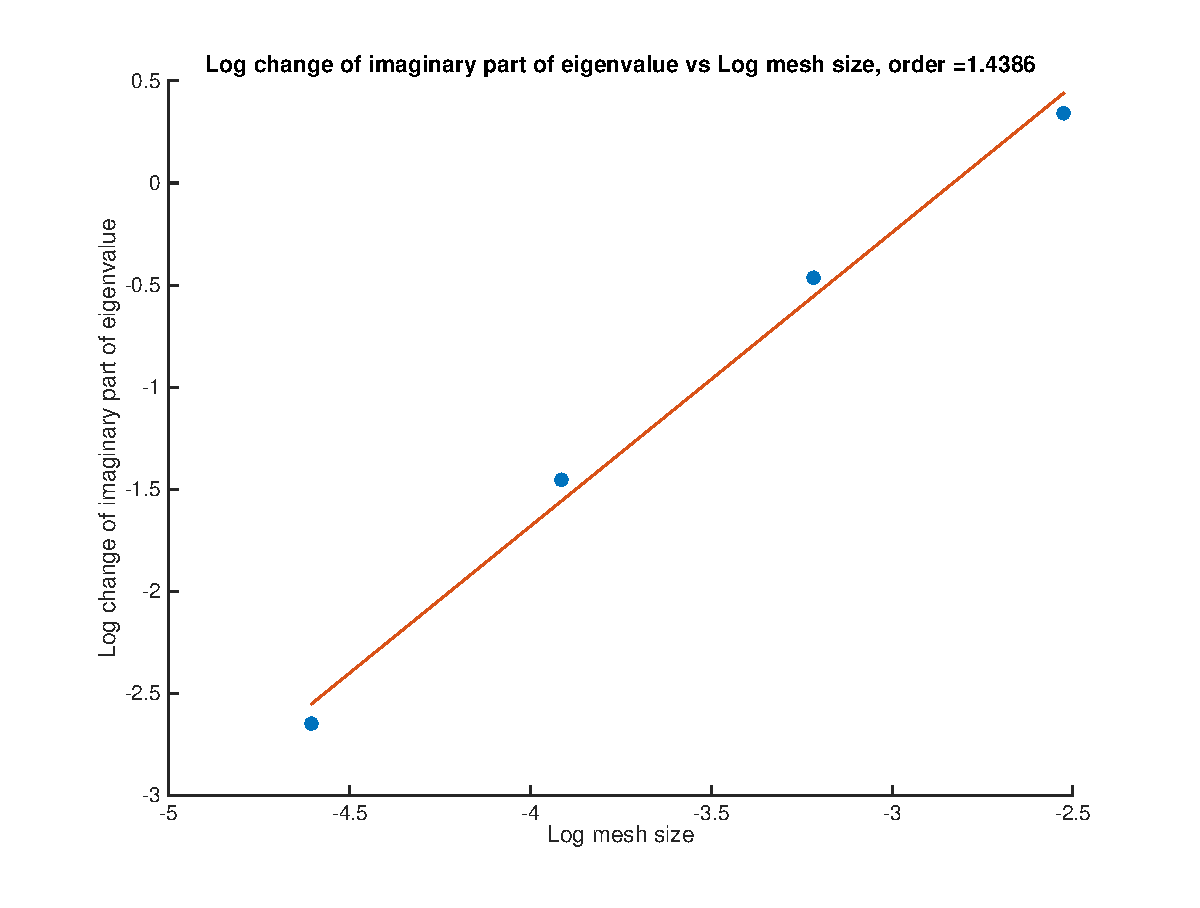
\includegraphics[width=8.5cm]{double2logplotleftimag.eps}
\end{figure}
Again, not the best, but an ok straight line. If we guess something like 0.61 for the imaginary part, we get the following graph.
\begin{figure}[H]
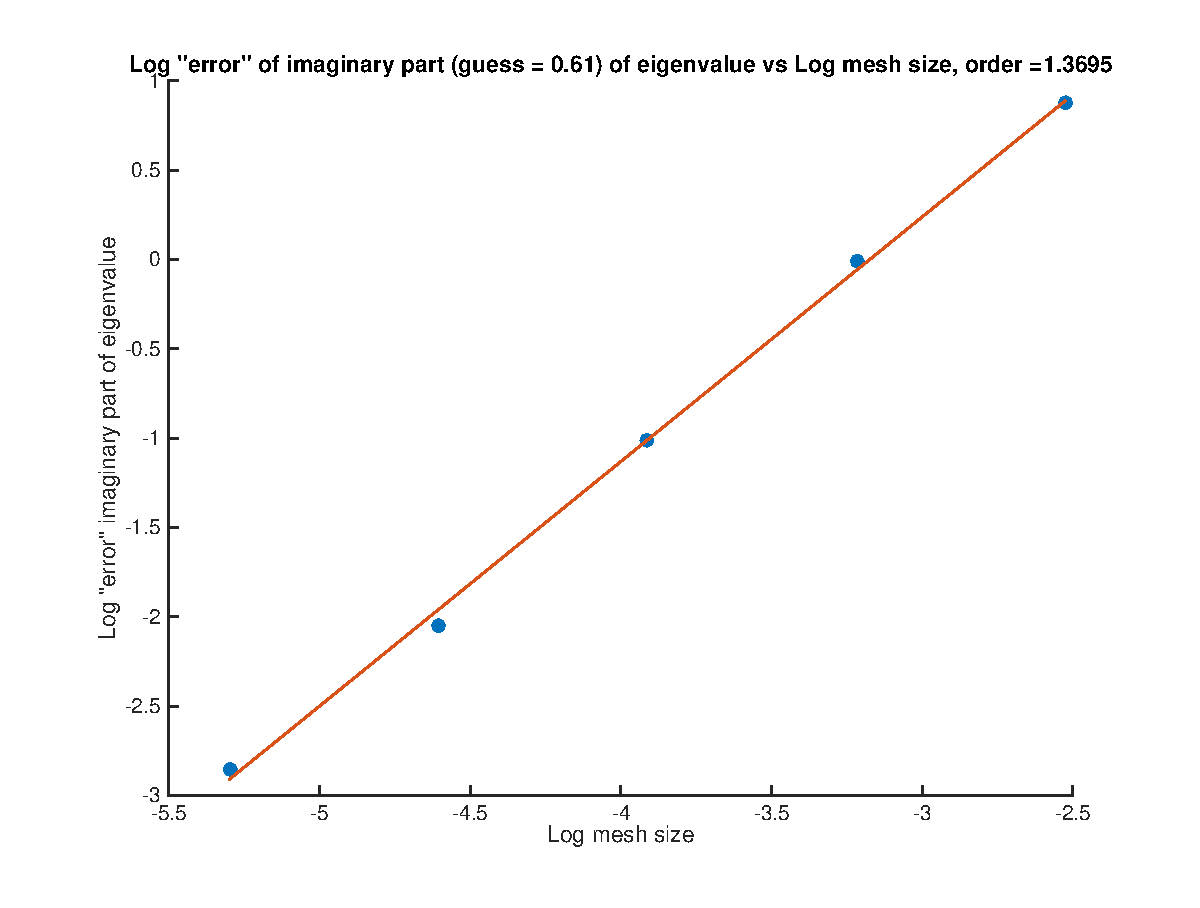
\includegraphics[width=8.5cm]{double2logplotleftimag2.eps}
\end{figure}

\subsubsection*{More data points}
To make this more convincing, we collect more data points to support our hypothesis that the real part of the left eigenvalue goes to 0 as the mesh size decreases to 0. Here is a log-log plot of the real part of the left eigenvalue versus mesh size for grid points from 6000 to 28000 (increments of 2000). We use exponential weight $a = 0.2$ to find these eigenvalues.
following graph.
\begin{figure}[H]
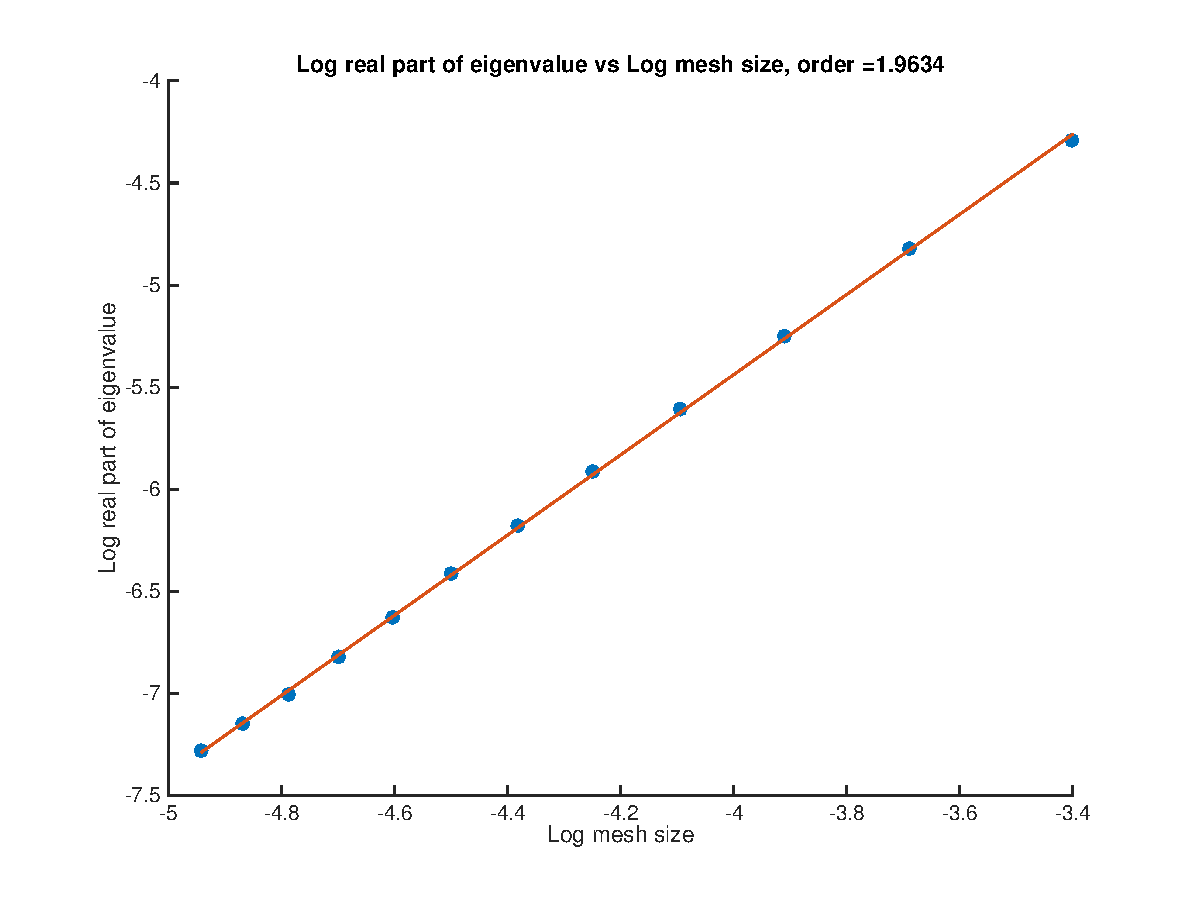
\includegraphics[width=8.5cm]{double2logplot3.eps}
\end{figure}
The straight line is much better, and the slope is approximately 2, which is the order of the finite difference scheme we are using. Thus by a numerical-methods-convergence argument, it seems reasonable to conclude that for Double Pulse 2, we have a pair of complex conjugate eigenvalues which are on the imaginary axis.\\

Just for comparison purposes, we do the same thing for the right eigenvalue, the one which should converge to 0. (Eigenfunction is the derivative of the double pulse.) Here are plots of the real part, imaginary part, and absolute value.
\begin{figure}[H]
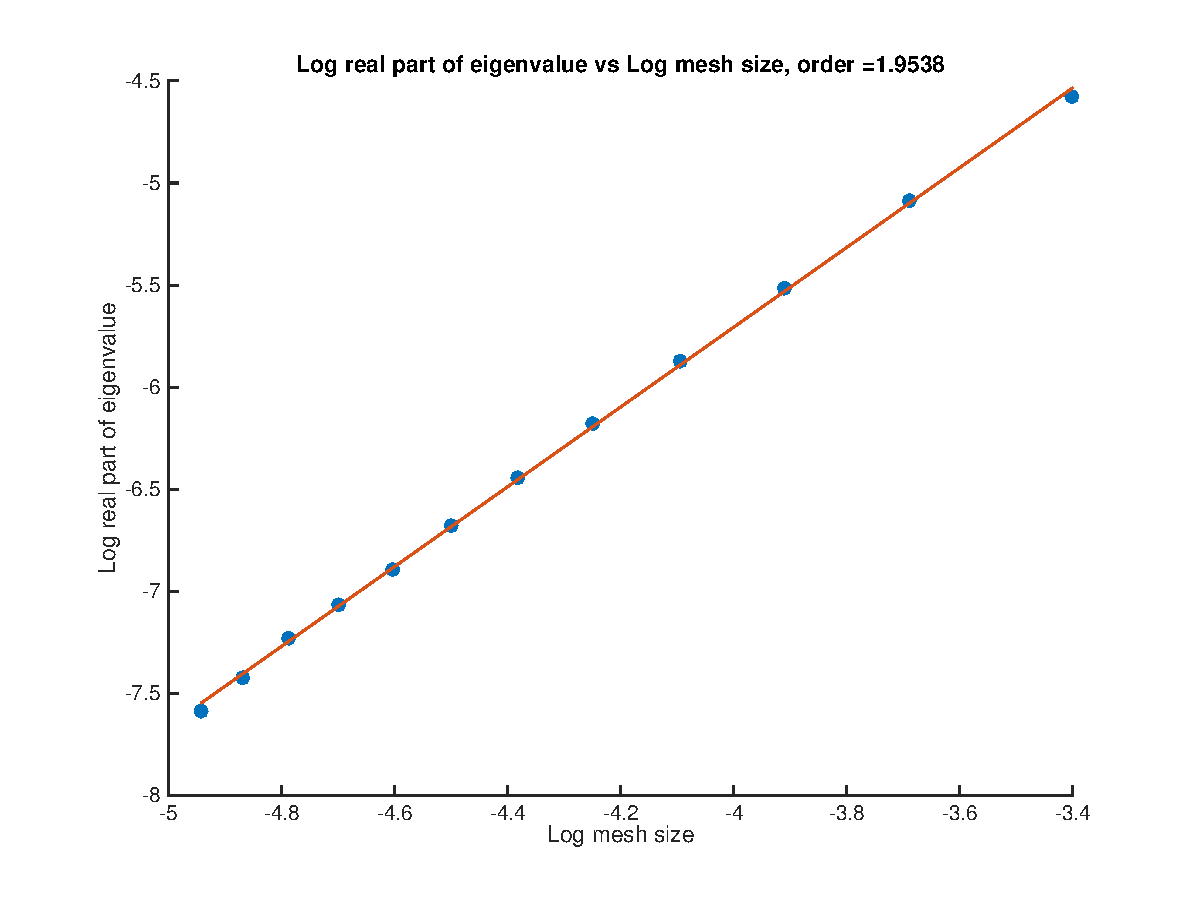
\includegraphics[width=8.5cm]{double2logplotright2real.eps}
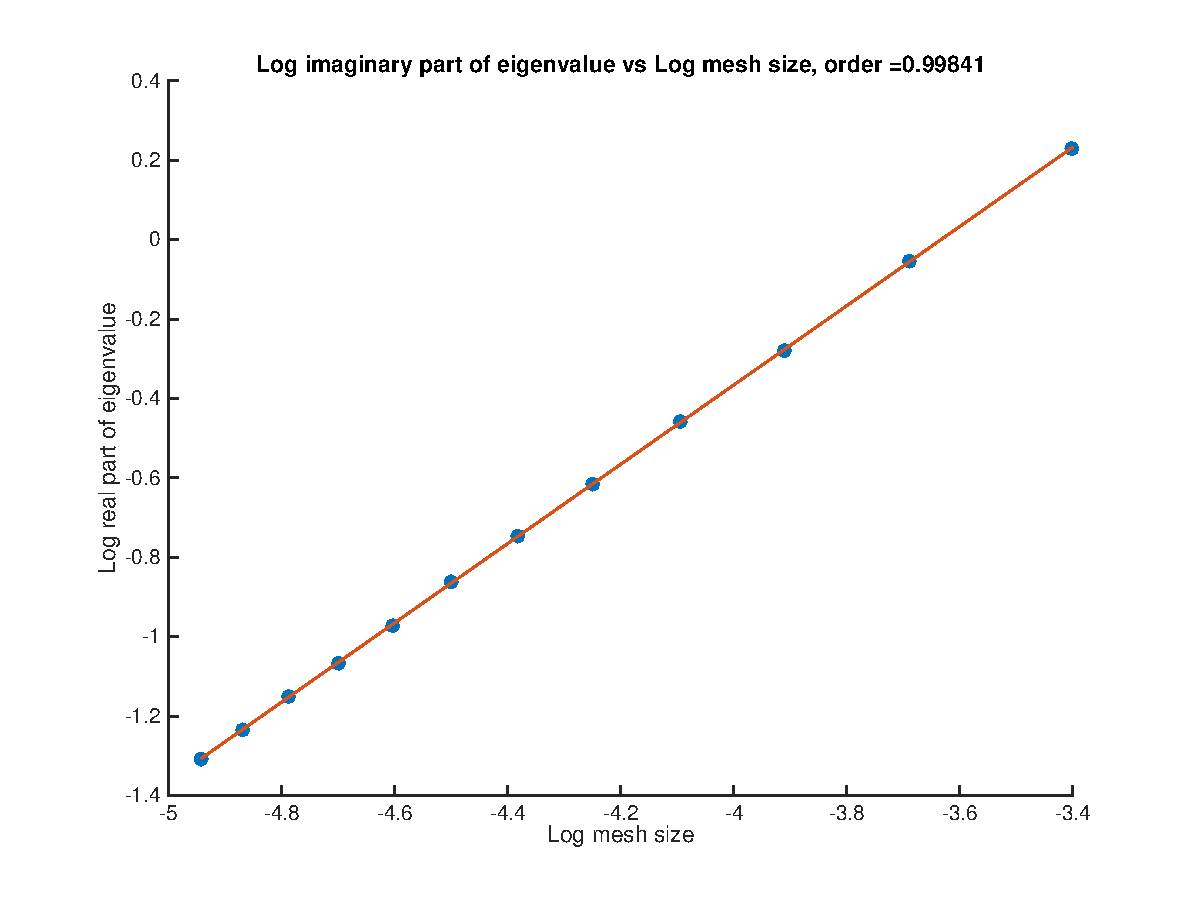
\includegraphics[width=8.5cm]{double2logplotright2imag.eps}
\end{figure}
\begin{figure}[H]
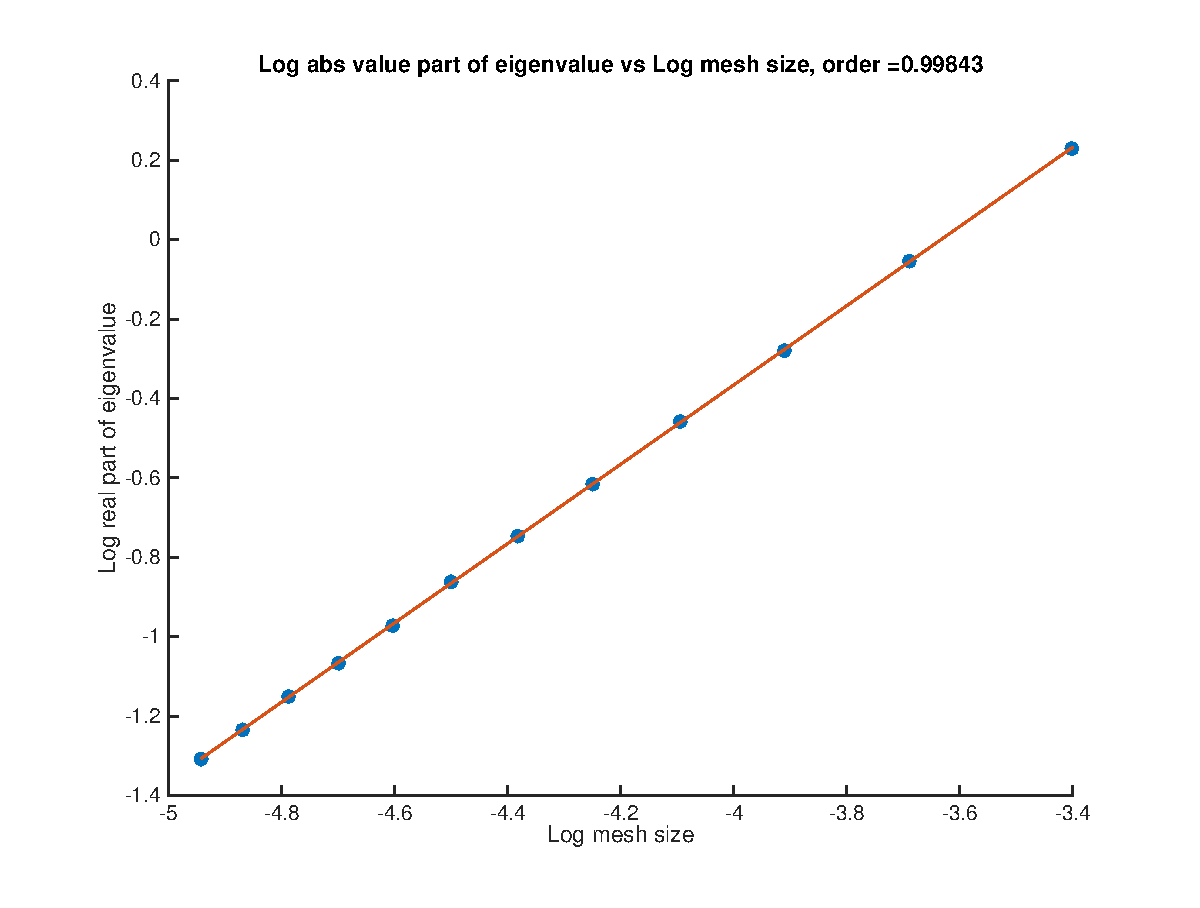
\includegraphics[width=8.5cm]{double2logplotright2abs.eps}
\end{figure}
Looking at the slopes of the graphs, the real part converges to 0 with order 2 (as did the left eigenvalue). The imaginary part convertes to 0 with only order 1. The absolute value converges to 0 with order 1 as well, which makes sense since it should follow the lower order of convergence. I have no idea why this should be the case.\\

If we repeat with Neumann BCs, we get the exact same result. Here is the plot showing the real part of the left eigenvalue converges to 0 with second order accuracy.

\begin{figure}[H]
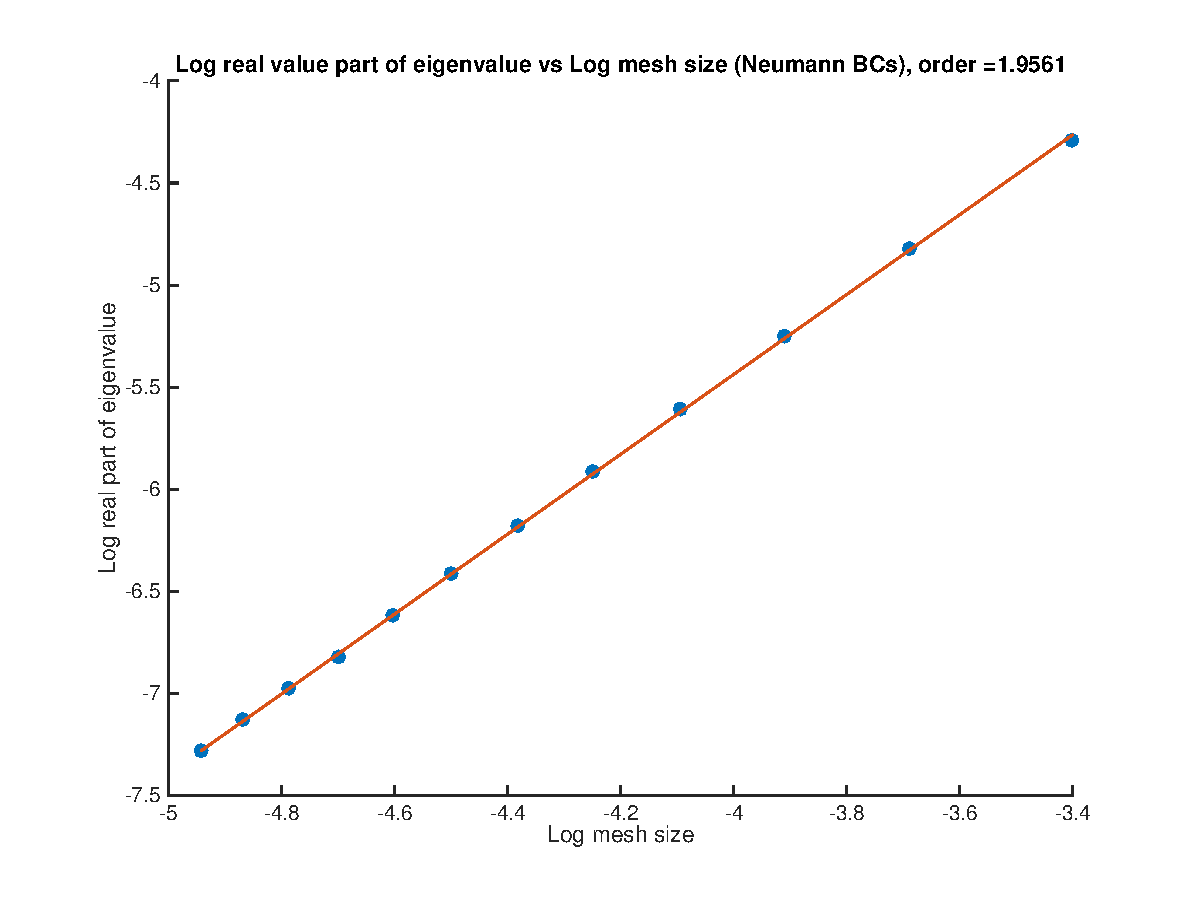
\includegraphics[width=8.5cm]{double2Neumannlogplot}
\end{figure}
The plots for the right eigenvalue are similar to the nes for periodic BCs above.

\subsubsection*{Repeat for different speed c}
If we repeat for a different speed $c = 18.6836$, we get the same results. We do the same thing as above, using the second double pulse and an exponential weight $a = 0.2$.

Table of eigenvalues:
\begin{figure}[H]
\begin{tabular}{l|ll}
$N$     & Left eigenvalue     &  Right eigenvalue  \\ \hline
        6000 &   -0.0040 + 0.4084i   & 0.0013 + 0.3574i \\ 
        8000 &   -0.0023 + 0.3321i   & 0.0008 + 0.2683i \\ 
       10000 &   -0.0015 + 0.2902i   & 0.0005 + 0.2147i \\ 
       12000 &   -0.0010 + 0.2647i   & 0.0004 + 0.1790i \\ 
       14000 &   -0.0008 + 0.2480i   & 0.0003 + 0.1534i \\ 
       16000 &   -0.0006 + 0.2366i   & 0.0002 + 0.1343i \\ 
       18000 &   -0.0005 + 0.2284i   & 0.0002 + 0.1194i \\ 
       20000 &   -0.0004 + 0.2224i   & 0.0001 + 0.1074i \\ 
       22000 &   -0.0003 + 0.2178i   & 0.0001 + 0.0976i \\    
\end{tabular}
\end{figure}

Here is a plot of the log of the real part of the left eigenvalue versus the log of the mesh size, where we see the real part goes to 0 as the mesh size decreases. The imaginary part does not go to 0, which we can see by looking at the table (through a little guesswork, it converges to somewhere near 0.18).
\begin{figure}[H]
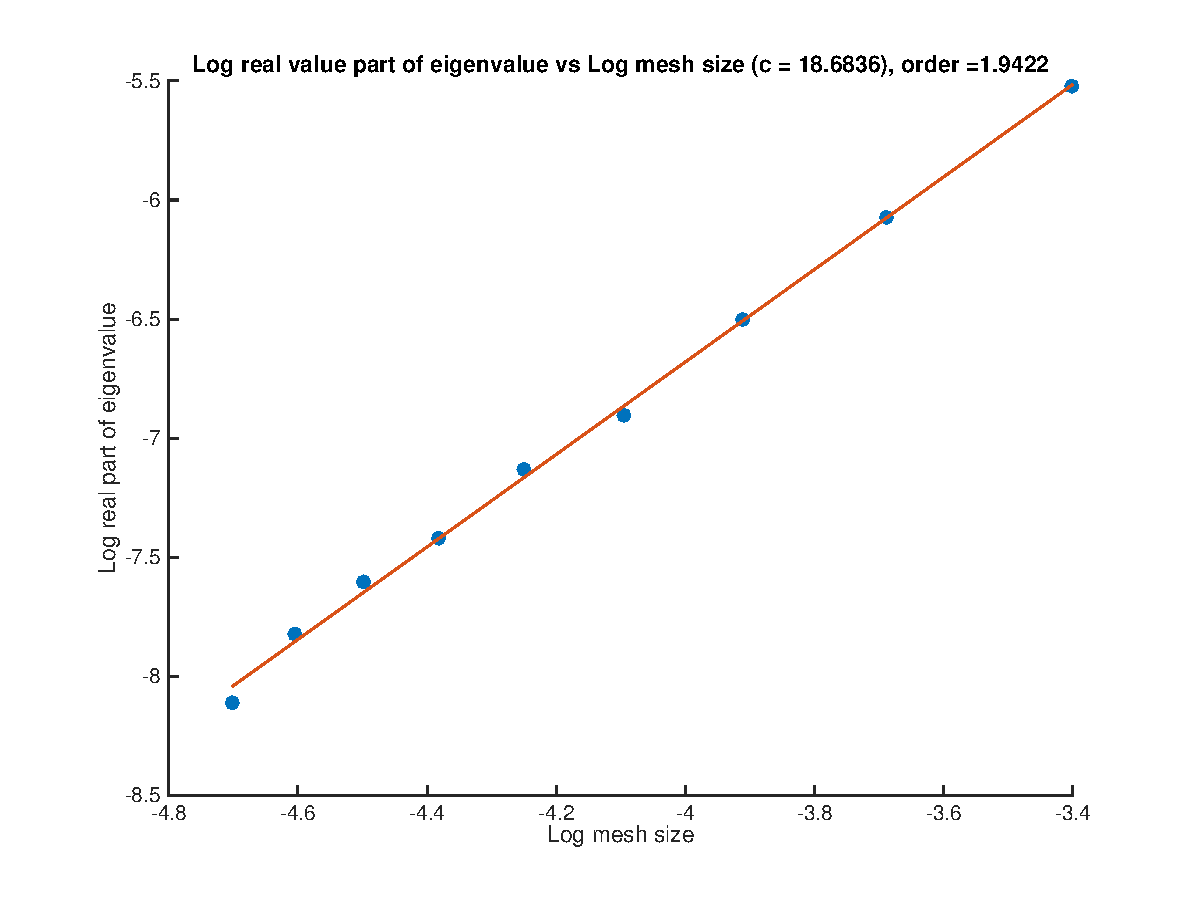
\includegraphics[width=8.5cm]{2double2logplot1}
\end{figure}
Here is a plot of the absolute value of the right eigenvalue versus the log of the mesh size, where we see the absolute value goes to 0 as the mesh size decreases.
\begin{figure}[H]
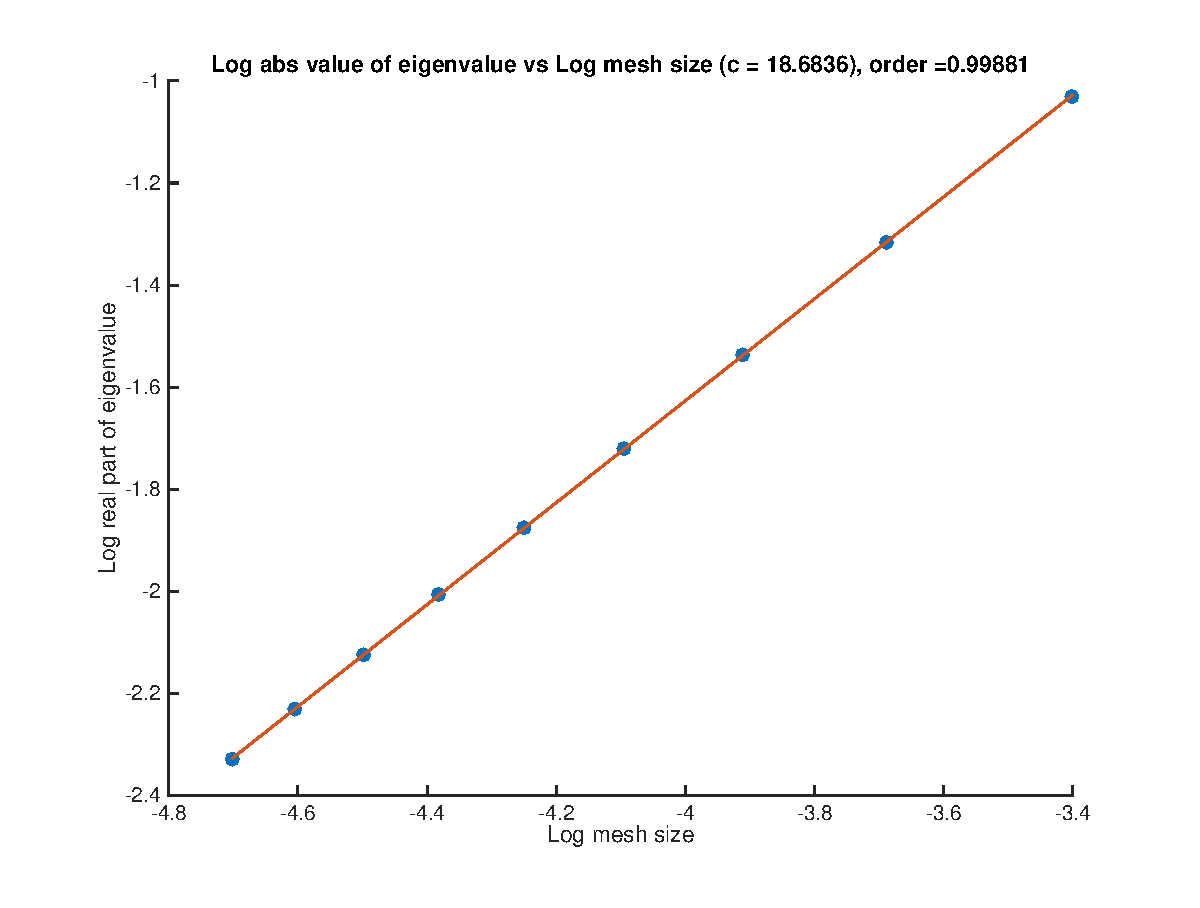
\includegraphics[width=8.5cm]{2double2logplot2}
\end{figure}

\end{document}

